\documentclass[]{article}
\topmargin -30pt \textheight 600pt \textwidth 500pt \oddsidemargin
10pt\evensidemargin 10pt



\usepackage[utf8]{inputenc}
\usepackage[english]{babel}
\usepackage{graphicx}
\usepackage{hyperref}
\usepackage{appendix}
\hypersetup{
	colorlinks=true,
	linkcolor=blue,
	filecolor=magenta,      
	urlcolor=cyan,
}
\usepackage{mathtools}
\usepackage{float}   %this package is for placing graphs and tables in where the TeX is
\graphicspath{{images/}{../images/}}

\usepackage{blindtext}

\usepackage{natbib}
\usepackage{subfiles}
\usepackage{verbatim}
\providecommand{\EqDir}{Equations}
\newtheorem{tm}{Theorem}
\newtheorem{dfn}{Definition}
\newtheorem{lma}{Lemma}
\newtheorem{assu}{Assumption}
\newtheorem{exam}{Example}
\newtheorem{claim}{Claim}
\newtheorem{prop}{Proposition}
\newcommand{\thm}{\begin{tm}}
\newcommand{\thmm}{\end{tm}}
\newcommand{\ex}{\begin{exam}}
\newcommand{\exx}{\end{exam}}
\newcommand{\lm}{\begin{lma}}
\newcommand{\lmm}{\end{lma}}
\newcommand{\cl}{\begin{claim}}
\newcommand{\cll}{\end{claim}}
\newcommand{\ass}{\begin{assu}}
\newcommand{\asss}{\end{assu}}
\newcommand{\df}{\begin{dfn}}
\newcommand{\dff}{\end{dfn}}
\newcommand{\prp}{\begin{prop}}
\newcommand{\prpp}{\end{prop}}
\newcommand{\eq}{\begin{equation}}
\newcommand{\eqq}{\end{equation}}
\newcommand{\bit}{\begin{itemize}}
\newcommand{\eit}{\end{itemize}}
\newcommand{\ben}{\begin{enumerate}}
\newcommand{\een}{\end{enumerate}}
\newcommand{\bqu}{\sloppy \small \begin{quote}}
\newcommand{\equ}{\end{quote} \sloppy \large}
\newcommand{\bcen}{\begin{center}}
\newcommand{\ecen}{\end{center}}
\newcommand{\nt}{\noindent}
\newcommand{\fn}{\footnote}

\begin{document}
\begin{titlepage}
\def\thefootnote{\fnsymbol{footnote}}
\vspace*{1.1in}
\title{Firm Entry and Exit: \\   \vspace{0.5em}
A Replication of Clementi-Palazzo (2016) and Khan-Thomas(2008)\fn{I am grateful to Prof. Chris Carroll for his encouragement and advice for replicating these papers. All remaining errors are my own.}}
\author{Aniruddha Ghosh}
\date{\today}

\end{titlepage}

\linespread{2}
\maketitle


\noindent  {\bf Abstract}: We analyze a simple version of Clementi and Palazzo (2016)’s \cite{cp16} model of the firm lifecycle (which
itself builds on Hopenhyan (1992) and Hopenhayn and Rogerson (1993)). The setup of it
replicates my code for Khan-Thomas. Further, we study the steady state of the model without aggregate
shocks. Further, we graph the results of our simulations.
    \hspace*{2.0em} 



\begin{small}
\parbox{\textwidth}{
\begin{center}
\begin{tabbing}
\texttt{~Archive:~} \= \= \url{http://econ.jhu.edu/people/ccarroll/BufferStockTheory.zip} \kill \\  %
\texttt{~~~~~PDF:~} \> \> \url{https://github.com/ani1231091/FirmEntryandExit/blob/master/Remark/Tex/main.pdf} \\
\texttt{~~Slides:~} \> \> \url{https://github.com/ani1231091/FirmEntryandExit/blob/master/Remark/Tex/Slides/Replication_Exercise.pdf} \\
\texttt{~~GitHub:~} \> \> \url{https://github.com/ani1231091/FirmEntryandExit} \\
\end{tabbing}
\end{center}
          }
\end{small}
\newpage

\section{Introduction}
Over the last 25 years, empiricists have pointed out a tremendous amount of between–firm
and between–plant heterogeneity, even within narrowly defined sectors. A key issue in
the macroeconomics literature is to gauge the importance of such heterogeneity for the
evolution of aggregate magnitudes. The objective of this paper is to assess the role that
entry and exit dynamics play in the propagation of aggregate shocks. The current exercise aims to complete the idiosyncratic version by modeling in aggregate shocks.  We analyse a model of lumpy investment wherein firms face persistent shocks to common and plant-specific productivity, and convex adjustment costs. The model extends the real business cycle model to include firm heterogeneity and fixed capital adjustment costs. The aggregate state vector of the model contains the distribution of firms over idiosyncratic productivity and capital, which evolves over time in response to aggregate productivity shocks. The dynamics of the distribution must satisfy a complicated fixed point problem: each firm’s investment decision depends on its expectations of the dynamics of the distribution, and the dynamics of the distribution depend on firms’ investment decisions. This infinite-dimensional fixed point problem is at the heart of the computational challenges faced by the heterogeneous agent literature.

\section{Related Literature}
Clementi-Palazzo(2016) are not the first to find that entry and exit enhance
the effects of aggregate shocks. Devereux, Head, and Lapham (1996), Chatterjee and
Cooper (2014), Bilbiie, Ghironi, and Melitz (2012), and Jaimovic and Floetotto (2008)
model entry and exit in general equilibrium models with monopolistic competition. In the
former three, a surge in entry leads to greater diversity of the product space. Because of
increasing returns, this encourages agents to work harder and accumulate more capital. In
Jaimovic and Floetotto (2008), more entry means more competition and lower markups.

Khan-Thomas(2008)'s setup is utmost useful for our project.
\section{Model}

\subsection{Firms}
We have two groups of firms. The first group of \textit{incumbent firms} behave similarly to Khan and Thomas (2008) model except that they have convex costs of capital adjustment rather than fixed costs. To be specific, each of these incumbent firms has a decreasing returns to scale production fucnction $$y_{jt}=e^{\epsilon_{jt}}k_{jt}^{\theta}n_{jt}^\nu$$, where $y_{jt}$ is output, $\epsilon_{jt}$ is idiosyncratic productivity, $k_{jt}$ is the firm's capital stock, $n_{jt}$ is the firm's labor input, and $\theta+\nu < 1$.

The idiosyncratic productivity $\epsilon_{jt}$ follows a Markov Chain process. Firms accumulate capital according to the accumulation equation $$k_{jt+1}=(1-\delta)k_{jt}+i_{jt}$$.

Capital accumulation incurs the convex adjustment cost $$-\frac{\varphi}{2} (\frac {i_{jt}}{k_{jt}})^2 k_{jt}$$, in units of output. At the beginning of each period, incumbent firms must pay a fixed cost $c_{f}$ units of output to remain in operation. A firm that does not pay this fixed cost does not produce, sells its entire capital stock with value $(1-\delta)k$ and permanently exits the economy.

There is a continuum of the second group of firms, the \textit{potential entrants}. These firms are ex-ante identical. At the beginning ofeach period, each firms decides whether to pay a fixed cost $c_{e}$ and enter the economy. If a potential entrant enters the economy, it draws a value for idiosyncratic productivity $\epsilon_{jt}$ from some distribution $\nu$ and begins as an incumbent firm with $k_{jt}=$0. We also assume that there are no adjustment costs at $k_{jt}=0$.

Further, we assume there is free entry among potential entrants, which implies that the exoected value from entering is less than or equal to the entry cost $c_{e}$, with equality if entry actually takes place. In equations, this condition is $c_{e} \leq \int v(\epsilon,0)\nu(d\epsilon)$, with equality if $m^{*} > 0$ (where $v(\epsilon,k)$ is the value function of an incumbent firm and $m^{*}$ is the mass of entrants in equilibrium.)



\subsection{Households}

Finally, there is a representative household with preferences over consumption $C_{t}$ and labor $N_{t}$ represented by the expected utility function

$$\mathrm E_{0} \sum_{t=0}^{\infty} \beta^{t}(log C_{t}- aN_{t})$$
where $\beta$ and $a$ are parameters. Output here is used for consumption, investment, capital adjustment costs, entry costs and operating costs. A steady state recursive competitive equilibrium of this economy is a set of incumbent value functions  $\nu(\epsilon,k)$. policy rules $k'(\epsilon,k)$ and $n(\epsilon,k)$, a mass of entrants per period $m^{*}$, a measure of active firms at the beginning of period $g^{*}(\epsilon,k)$ and real wage $w^{*}$ such that 

\begin{itemize}

\item incumbent firms maximize their firm value;

\item the free entry condition holds;

\item the labor market clears;

\item the measure of active firms $g^{*}(\epsilon,k)$ is stationary.

\end{itemize}

More formally, let me define the recursive equilibirum now.

\section{Recursive Equilibrium}

At the beginning of each period, incumbent firms must pay a fixed cost \( c_{f} \) units of output to remain in operation. A firm that does not pay this fixed cost permanently exits the economy immediately and sells its entire capital stock with value \( (1-\delta) k, \)
i.e. \( V_{x}(k)=(1-\delta) k \). 

Then, the start-of-period value of an incumbent firm is dictated by the function \( V(\lambda, k, s) \) which solves the following functional equation:
\[ V(\varepsilon, k)=\max \left\{V_{x}(k), \tilde{V}(\varepsilon, k)-c_{f}\right\} \] Given that firms accumulate capital according to the accumulation equation \( k_{j t+1}= \) \( (1-\delta) k_{j t}+i_{j t} \) and capital accumulation incurs the adjustment cost \( -\frac{\varphi}{2}\left(\frac{i_{jt} }{k_{j t}}\right)^{2} k_{j t} \), in units of output. The prospective value of an entrant is \[ V(\varepsilon, 0)=\max \left\{0, \tilde{V}(\varepsilon, 0)-c_{e}\right\} \] hence, she will invest and start operating if and only if \( c_{e} \leq \int V(\varepsilon, 0) d \varepsilon \)
For a given Markov process, a recursive competitive equilibrium consists of
(i) value functions \( V(\varepsilon, k), \bar{V}(\varepsilon, k) \) and \( V_{e}(\varepsilon, 0), \);
(ii) policy functions \( n(\varepsilon, k), k^{\prime}(\varepsilon, k), \);
(iii) bounded sequences of wages \( \left\{w_{t}\right\}_{t=0}^{\infty}, \) incumbents' measures \( \left\{g_{t}\right\}_{t=1}^{\infty}, \) and entrants' measures \( \left\{m_{t}\right\}_{t=0}^{\infty} \) such that, for all \( t \geq 0 \).

1. \( V(\varepsilon, k), \tilde{V}(\varepsilon, k), \) and \( n(\varepsilon, k) \) solve the incumbent's optimization problem;

2. \( V_{e}(\varepsilon, 0) \) and \( k^{\prime}(\lambda, 0) \) solve the entrant's optimization problem;

3. The representative houschold chooses consumption and labour such that \( \frac{w(g)}{C(g)}= \) \( \frac{a}{N(g)} \);

4. The labour market clears: \( N\left(w_{t}\right)=\int n\left(\varepsilon_{t}, k\right) g_{t}(\varepsilon, k) d \varepsilon d k \forall t \geq 0 \);

5. The goods market clears: \( C\left(g_{t}\right)=\int\left[y\left(\varepsilon_{t}, k\right)-i\left(\varepsilon_{t}, k\right)\right] g_{t}(\varepsilon, k) d \varepsilon d k: \forall t \geq 0 \).

\begin{center}
 \begin{tabular}{ | c |  c |  c | }
\hline
 Parameter & Description & Value \\ [0.5 ex]
\hline \hline
 $\beta$ & Discount Factor & .961 \\
\hline
$\varphi$ & Convex Cost adjusment & .5 \\
 $\sigma$ & Utility curvature & 1 \\
 $\alpha$ & Inverse Frisch & lim $\alpha \rightarrow$ 0 \\
 $\chi$ & Labor Disutility & N*$=\frac{1}{3}$ \\
 $\nu$ & Labor Share & 0.64 \\
 $\theta$ & Capital Share & 0.21 \\
 $\delta$ & Capital Depreciation  &  0.1  \\
 $\rho_{z}$ & Idiosyncratic TFP AR(1) &  0.859 \\
 $\sigma_{z}$ & Idiosyncratic TFP AR(1) &  0.02 \\
 $n_{ss}$ & Steady State Labor & 0.6 \\
$c_{f}$ & Incumbent's cost & 0.01 \\
$c_{e}$ & Entrant's cost & 0.02 \\
$m$ & Tauchen Grid initializer & 3 \\
\hline
\end{tabular}    
\end{center}


\subsection{Representative Agent Steady State}
We begin by analysing the steady state equilibrium of the model in which there is a representative firm and productivity is equal to the mean value of \( \varepsilon \). In this scenario, the steady state recursive competitive equilibrium is characterized by a set \( V^{*}(\bar{\varepsilon}, k), C^{*}, N^{*}, w^{*} \) and \( g(\bar{\varepsilon}, k)^{*} \) such that
1. \( V^{*}(\bar{\varepsilon}, k) \) solves the representative firm's optimization problem (i.e. Bellman eq.);
2. Taking \( N^{*} \) as given, the representative household's optimization is satisfied by \( \frac{w^{*}}{C^{*}}=\frac{a}{N^{*}} \)
3. Labour market clearing follows from \( N^{*}\left(w_{t}\right)=\int n(\bar{\varepsilon}, k) g(\bar{\varepsilon}, k) d k \forall t \geq 0 \)
4. The goods market satisfies \( C^{*}=\int[y(\bar{\varepsilon}, k)-i(\bar{\varepsilon}, k)] g(\bar{\varepsilon}, k) d k \forall t \geq 0 \)

Now, assume that steady state labour supply is \( N_{r e p}^{*}=0.6 . \) Then, we can use the following system of equations to solve for \( K_{r e p}^{*} \) and \( w_{r e p}^{*}=0.6 . \) Then, we can use the \[ \bar{n}=0.6 \]
\( \bar{r}=\frac{1}{\beta}-(1-\delta) \)
\( \bar{k}=\frac{1}{\beta}-(1-\delta) \)
\( \bar{k}=\delta \bar{k} \)
\( \bar{i}=\nu \bar{k} \)
\( \bar{w}=\nu \bar{k}^{\theta} \bar{n}^{\nu-1} \)
\( \bar{c}=\bar{k}^{\theta} \bar{n}^{\nu}-\bar{i} \)
\( \bar{a}=\frac{w^{*} n^{*}}{c^{*}} \)

In particular, \( K_{r e p}^{*}=1.09 \) and \( w_{r e p}^{*}=0.78 . \)


\section{Some plots}
\begin{figure}[H]
          \caption{Firm Distribution}
	\centering
	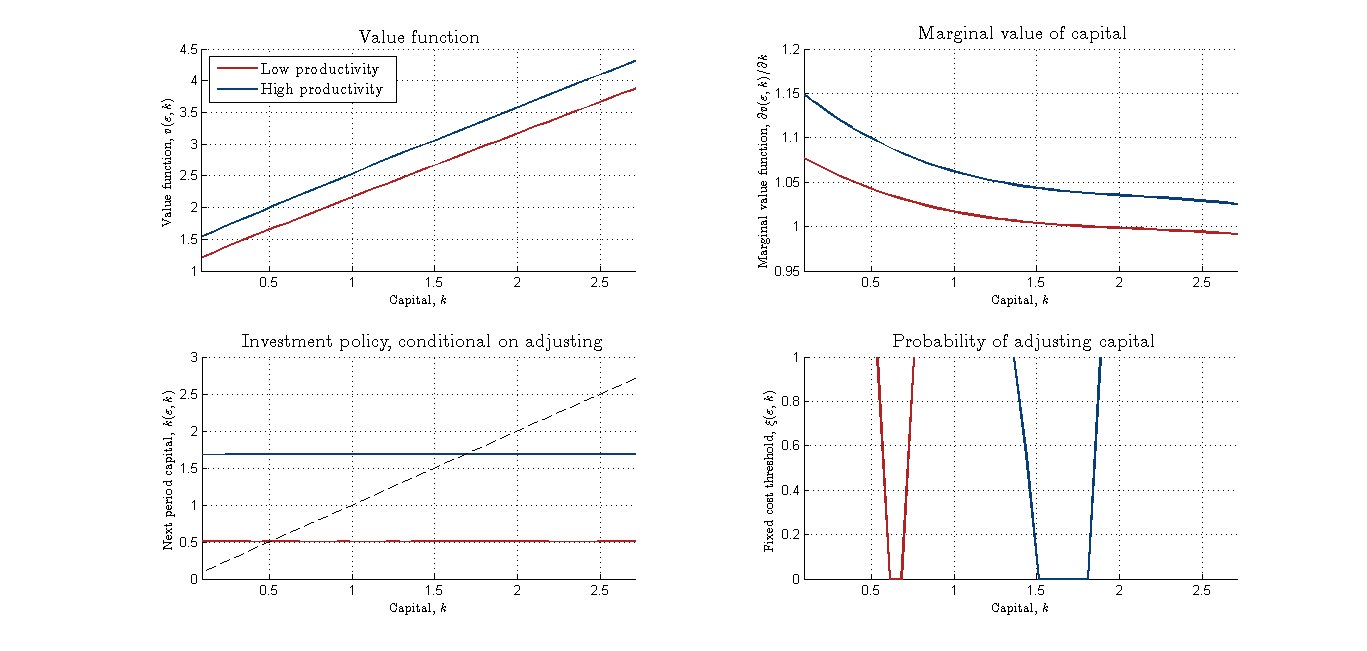
\includegraphics[scale=0.5]{Figures/Vf-1}
	\label{figure:1}
\end{figure}

\begin{figure}[H]
	\caption{Marginal Product Distribution}
            \centering
	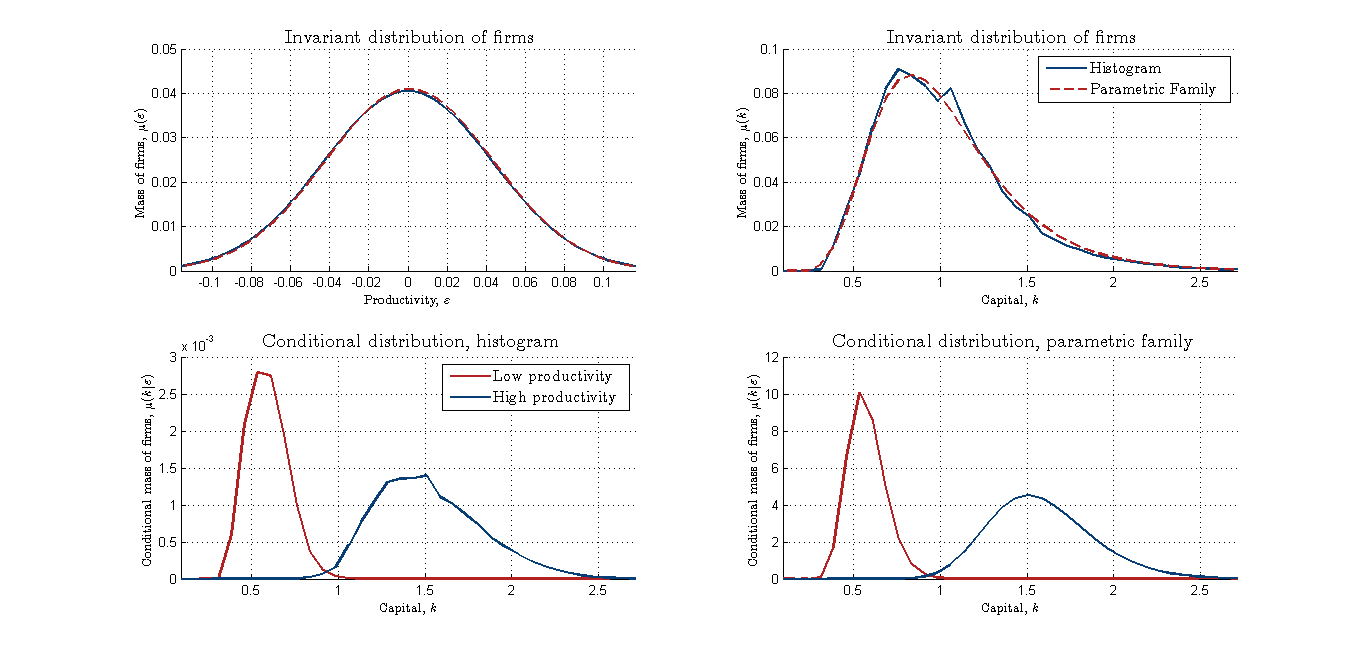
\includegraphics[scale=0.5]{Figures/Vf-2}
	\label{figure:1}
\end{figure}

\begin{figure}[H]
	\centering
	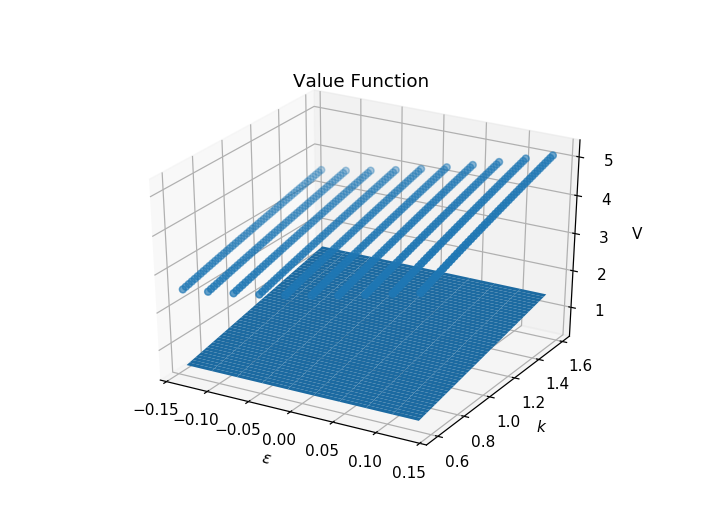
\includegraphics[scale=0.5]{Figures/Vf-3}
	\label{figure:1}
\end{figure}

\begin{figure}[H]
	\centering
	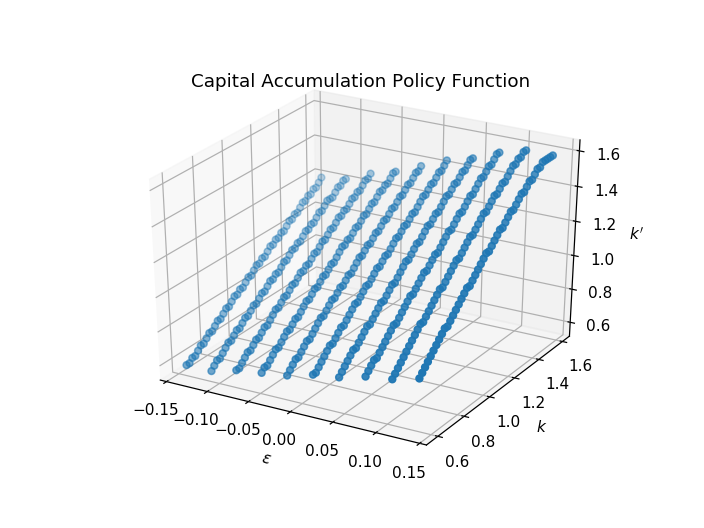
\includegraphics[scale=0.5]{Figures/Vf-4}
	\label{figure:1}
\end{figure}

\begin{figure}[H]
	\centering
	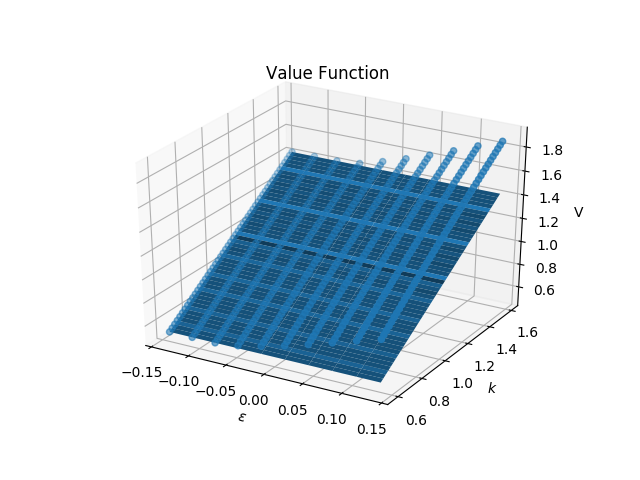
\includegraphics[scale=0.5]{Figures/VF-5}
	\label{figure:1}
\end{figure}

\begin{figure}[H]
	\centering
	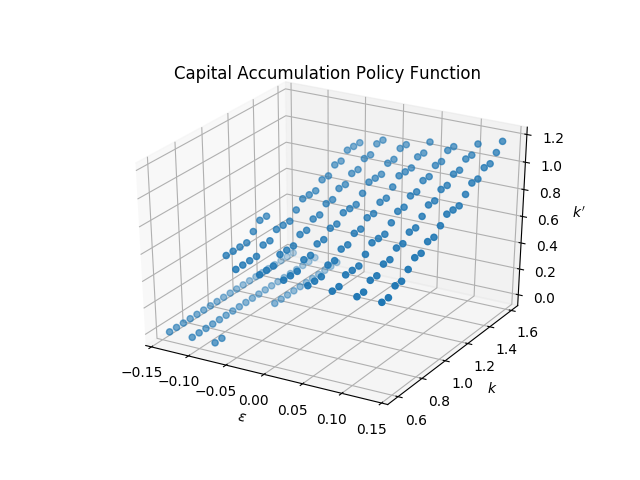
\includegraphics[scale=0.5]{Figures/Vf-6}
	\label{figure:1}
\end{figure}

\begin{figure}[H]
	\centering
	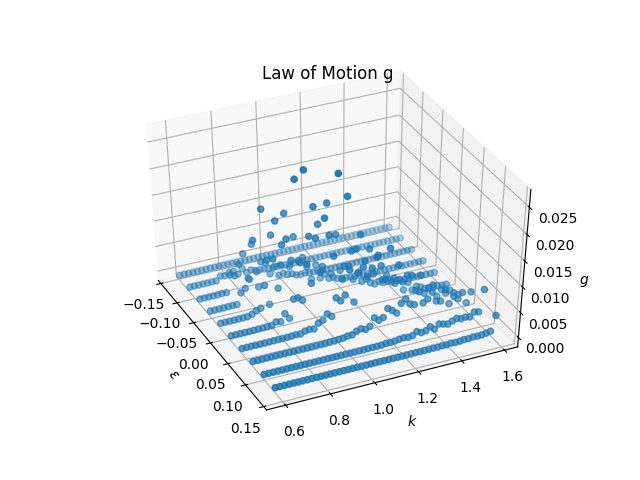
\includegraphics[scale=0.5]{Figures/Vf-7}
	\label{figure:1}
\end{figure}

\begin{figure}[H]
	\centering
	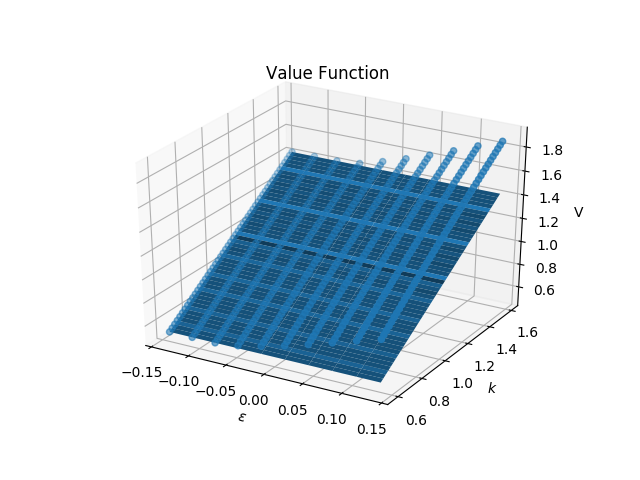
\includegraphics[scale=0.5]{Figures/Vf-8}
	\label{figure:1}
\end{figure}

\newpage

\section{Appendix}{\label{Appendix}}
	\subfile{Appendix/Appendix}

\newpage

\bibliography{References/Clementi-Palazzo}


\end{document}
